\chapter{Arquitechture}
\label{chap:architecture}

\begin{chapterintro}

In this section, we describe the overall architecture of a QA system that features social dialog in a learning environment.
 
\end{chapterintro}

\cleardoublepage

\section{Overview of the modules}

As already stated, in this section we will describe the architecture of our system, starting with the modules identified in the requirements. This requirements are:
\begin{enumerate}[noitemsep, label=(\roman*)]
 \item Present the user with a simple interface for their questions, and to present them with the answers.
 \item Classify each input according to the speech act it performs.
 \item Track dialog options according to the speech.
 \item Implement a QA system being able to search the document library and extract a short answer.
 \item Extend the documents library, scrapping external documents and producing semistructured indexes.
 \item Follow up the learning process, and use it to improve the learning experience. 
\end{enumerate}

In figure \ref{fig:arch1} we show the global architecture of the system, identifying four main modules: Conversational Agent, Teaching Agent, Question Answering and Information Extraction Agent. In the rest of this section we will discuss the function of reach module.

\color{red}\emph{Añadir info sobre el clasificador?}\color{black}


\begin{figure}[!htbp]
    \centering
    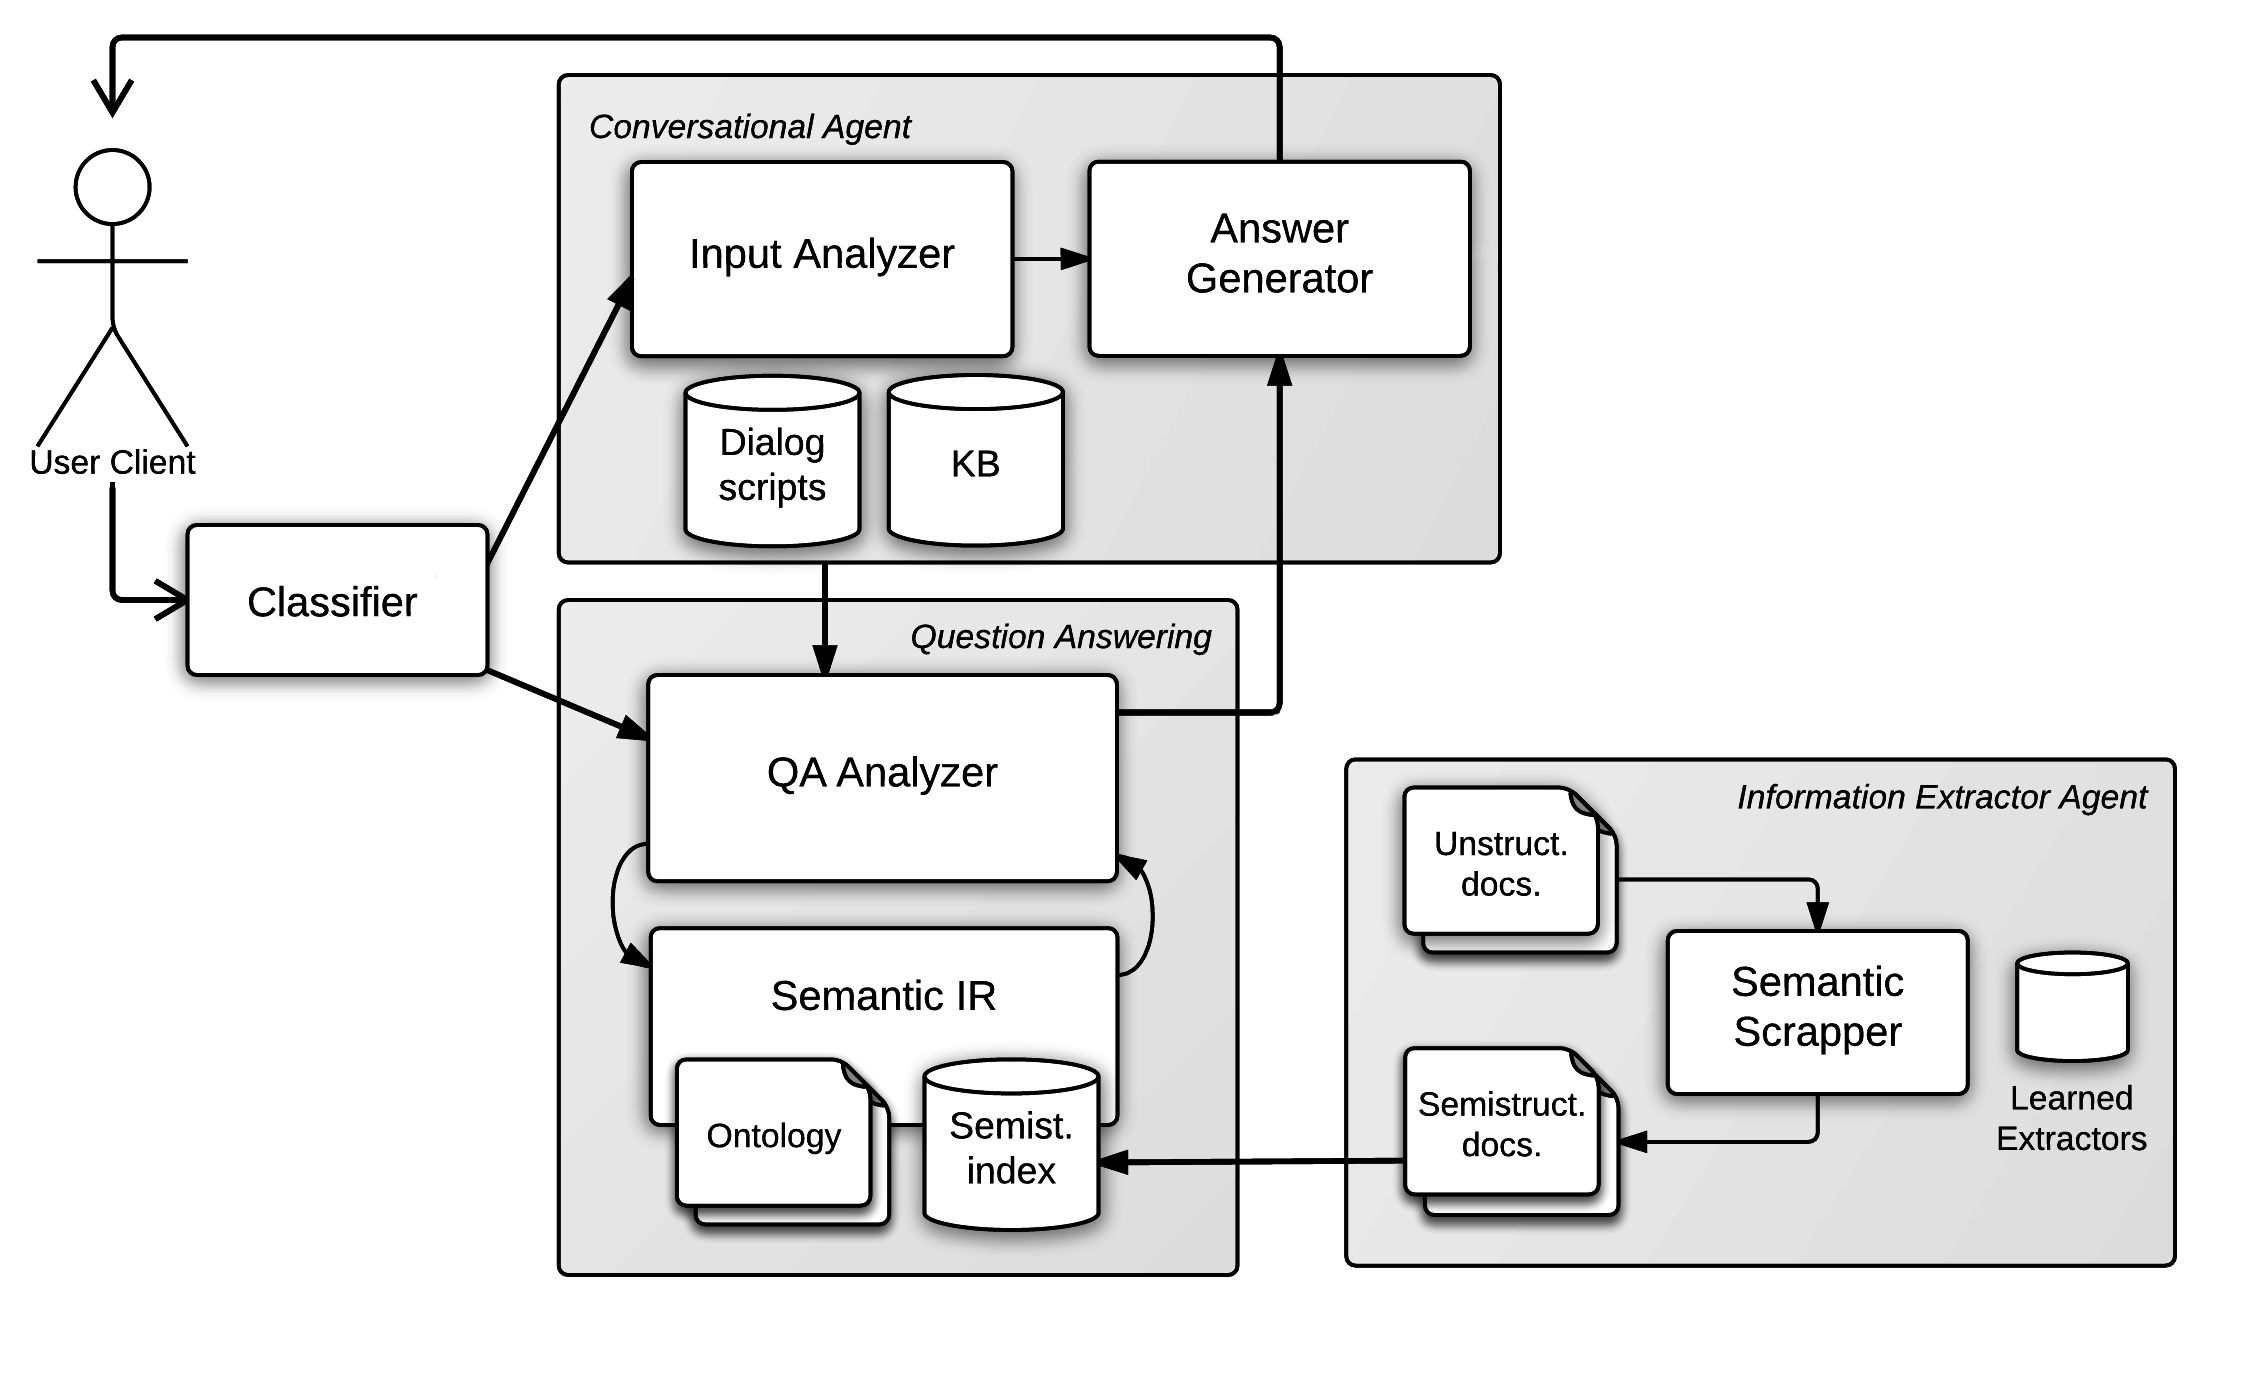
\includegraphics[width=0.7\textwidth]{img/arch/global_1-3.png}
    \caption{Global view of the architecture proposed}
    \label{fig:arch1}
\end{figure}



\subsection{Conversational Agent}

The {\em Conversational Agent} is responsible for handling the social dialog of the conversation (also referred by other authors as small talk or chit chat). It also traces the topic of the conversation that stores in the fact \ac{KB}, along with the former utterances and pills of information learned or devised from the user. It is responsible for understanding the whole meaning of the user query when he/she omits information already provided in previous utterances. 
The Input Analyzer inside the Conversational Agent, performs a script based analysis of the input by matching regular expressions against the input. Some advanced implementations of script based analyzers also use dictionaries and perform \ac{PoS} tagging and parsing.

The Conversational Agent, by means of the Answer Generator, is also in change of generating the answers that will be sent to the users. These are also stored in the dialog scripts. 
In the most common scenario, the small talk input is analyzed by the Input Analyzer and tells the Answer Generator to given a particular answer in response.
However, the \ac{QA} and the Teaching Agent modules can also instruct the Answer Generator to send a response to the user.
In those cases, the Conversational Agent generates the answer according to the topic and former utterances, giving it a particular touch when needed.
Besides the textual response that is presented to the user, the answer is decorated with metadata to provide further information about the state of the Conversational Agent. Typically, they indicate the mood of the agent, its facial expressions and gestures (possible implemented using \ac{BML}), etc.


\subsection{Question Answering}

The {\em Question Answering} takes part with those user queries where he/she asks for a particular piece of information, i.e. as with a regular \ac{QA} system. 
The QA Analyzer uses domain-specific grammars to extract the precise meaning of the query.
This is, it is classifies the type of query, extracts the relevant concepts, and categorize them according to the ontologies considered. The effectiveness of the process depends of the accuracy and degree of detail of the grammars applied, which includes the precision of the concept categorization. The QA Analyzer combines general-scope dictionaries with domain-specific ones to enhance its effectiveness. If there is no grammar that can be applied to the query, the analysis simply does not return any outcome.

As with regular \ac{QA} systems, the \ac{IR} is consulted to obtain the relevant documents where the answer is contained. The \ac{IR} works with a set of documents that has been previously indexed.
% Once the user query is analyzed the system decides whether the system needs to query the available document in order to retrieve the information to generate the results. 
In this case, given the semantic nature of the \ac{IR} system, it also acts as a SPARQL endpoint that may be queried for precise pieces of information. Thus, it supports a dual working mode depending on the nature of the query. 
With semantic queries the results are more precise and the information returned has better structure, the better categorization of the fields returns the more accurate results. 
Semantic queries also enable the use of linked data not only for enhancing results but for query expansion.
% {\bf search som QueryExpansion papers or review those at mendeley}. 
When the semantic IR is not available --either because the incoming query is too general, or because there is no relevant structured documents--, the IR module will do its best to return a piece of information as accurate as possible. At least, it retrieves a set of documents that are related to the query. It will try to categorize the nature of the documents, which bring the category of the concept searched, that can be used to expand the query and reformulate the query.
%  The main advantage of including semantic IR is that it will provide a result, depending on the quality of the documents, the quality of the result may vary, but in most cases (but when there is no relevant document at all) it will produce a result.
If no relevant document is returned by the \ac{IR}, the \ac{QA} is not capable to give a response, and thus the Answer Generator will inform the user. 

Moreover, the Semantic \ac{IR} may also be queried by external modules, e.g. the Teaching Agent. The treatment given to the query is the same as when it comes from the QA Analyzer.
Finally, the conversational agent may derive a query to the \ac{QA} in those cases where the Speech Act Classifier missclassifies the query, and more frequently with those utterances where the user	 asks for more information. In this case, the \ac{QA} system needs further information to perform the document retrieval. Thus, the conversational agent will expand the query and route it to the \ac{QA}.


\subsection{Information Extractor}

In case there is no relevant document for the query performed, the system will try update the KB. The {\em Information Extractor Agent}'s main function consists on analyzing unstructured documents in order to extract fields, categorize them and generating a semistructured document. 

This is a slow process, so it cannot be performed in near real-time; instead, unresolved query may trigger its execution, that will be available for future queries. 
This automatic information extraction mechanism is a best-effort process that relies on the information on the sources, and the ontologies used to map that information. Semantic scrappers such as Scrappy~\cite{villamor13} may boost this process.
Alternatively, a system administrator may also manually include documents on the \ac{IR} index, but also mark them to be processed by the Information Extractor Agent and index them afterwards.

\subsection{Teaching agent}

The {\em Teaching Agent} supervises the learning process of the users, and is in charge of improving their learning experience.
To do so, it  gathers information about all interactions of the user with the system. This information is obtained from the \ac{KB} of the Conversational Agent (or derived from it) which is synchronised with the Student Profile KB of the \ac{ITS}.
An \ac{ITS} is usually implemented as a \ac{MAS} of \ac{BDI} agents. In that case, the Student Profile KB is included in the \ac{BB} of the agent. 

% I don't really know if this should go here or not...
%\section{Prototype}
%
\section{Work process} % Revise this title

In this section we will describe the process a question introduced into the system will follow. Depending on the user input, the aforementioned process may differ. Here, we will consider two types of user input, the first one being a simple chit chat sentence, that won't require a look up in the \ac{KB}. The other type of input to be considered is an actual question, requiring a lookup in the \ac{KB}.

% Add UML figure?

The classifier will differentiate between the different types of input, and trigger the appropriate processes.

\subsection{Simple sentence}

Our system is ready to handle social chat, which aims to provide a richer experience to the user, encouraging him to keep chatting and having a better learning experience. In this case, a \ac{KB} lookup is not required, and therefore, the process is as stated:

\begin{enumerate}
 \item The user inputs the sentence into the system.
 \item The classifier tags the input as chit-chat.
 \item The input analyzer decides which type of social interaction we are facing, such as a greeting, a identifying question (``Are you the teacher? `` ) or an insult, among others.
 \item The answer generator provides an appropriate response and returns it to the user.
\end{enumerate}

This process is shown graphically in Figure \ref{fig:arch2}

\begin{figure}[!htbp]
    \centering
    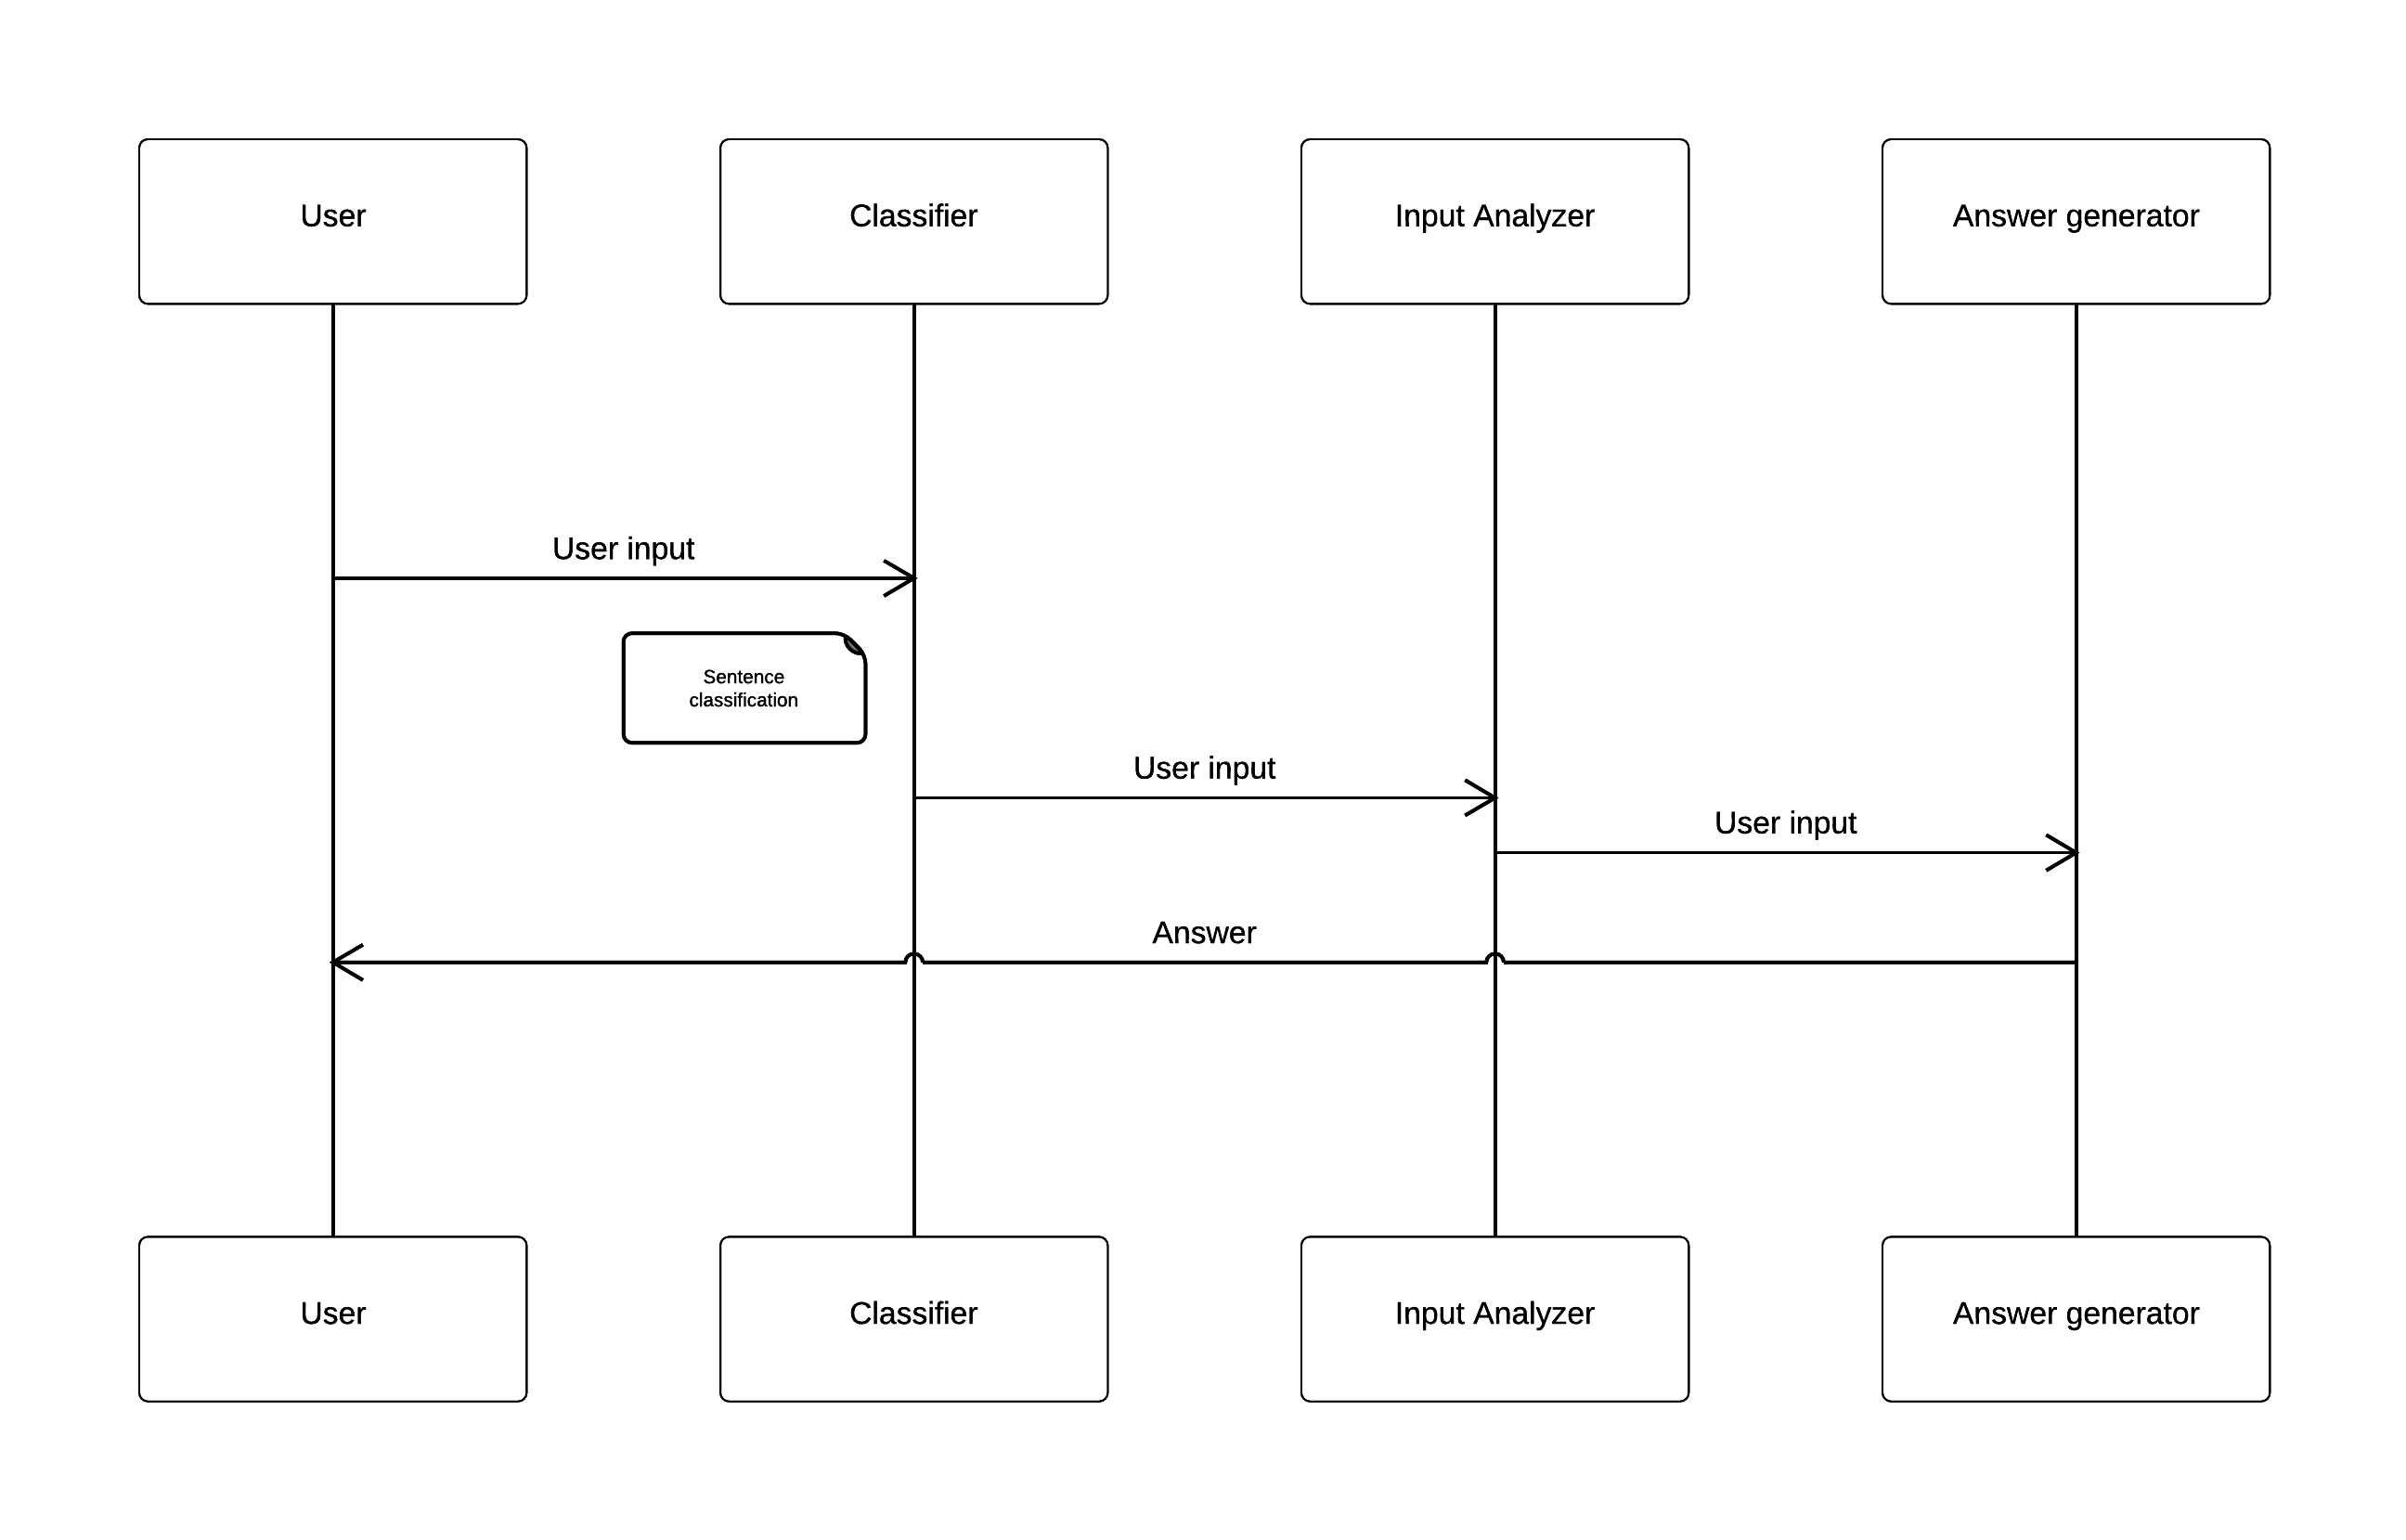
\includegraphics[width=\textwidth]{img/arch/SimpleSentence.png}
    \caption{Simple sentence process}
    \label{fig:arch2}
\end{figure}

\subsection{Question with \ac{KB} lookup}

In this process, the question input into the system does require a lookup in the \ac{KB}, via the \ac{QA} system. The process followed to produce the output will be the following:

\begin{enumerate}
 \item The user inputs the question into the system.
 \item The classifier tags the input as an actual question.
 \item The QA Analyzer process the question and performs a search in the \ac{KB}.
 \item The QA Analyzer returns the response for the question to the Answer generator.
 \item The answer generator process the response and returns a natural question, as well as the required \ac{OoB} command with the data.
\end{enumerate}

Figure \ref{fig:arch3} shows the process graphically.

\begin{figure}[!htbp]
    \centering
    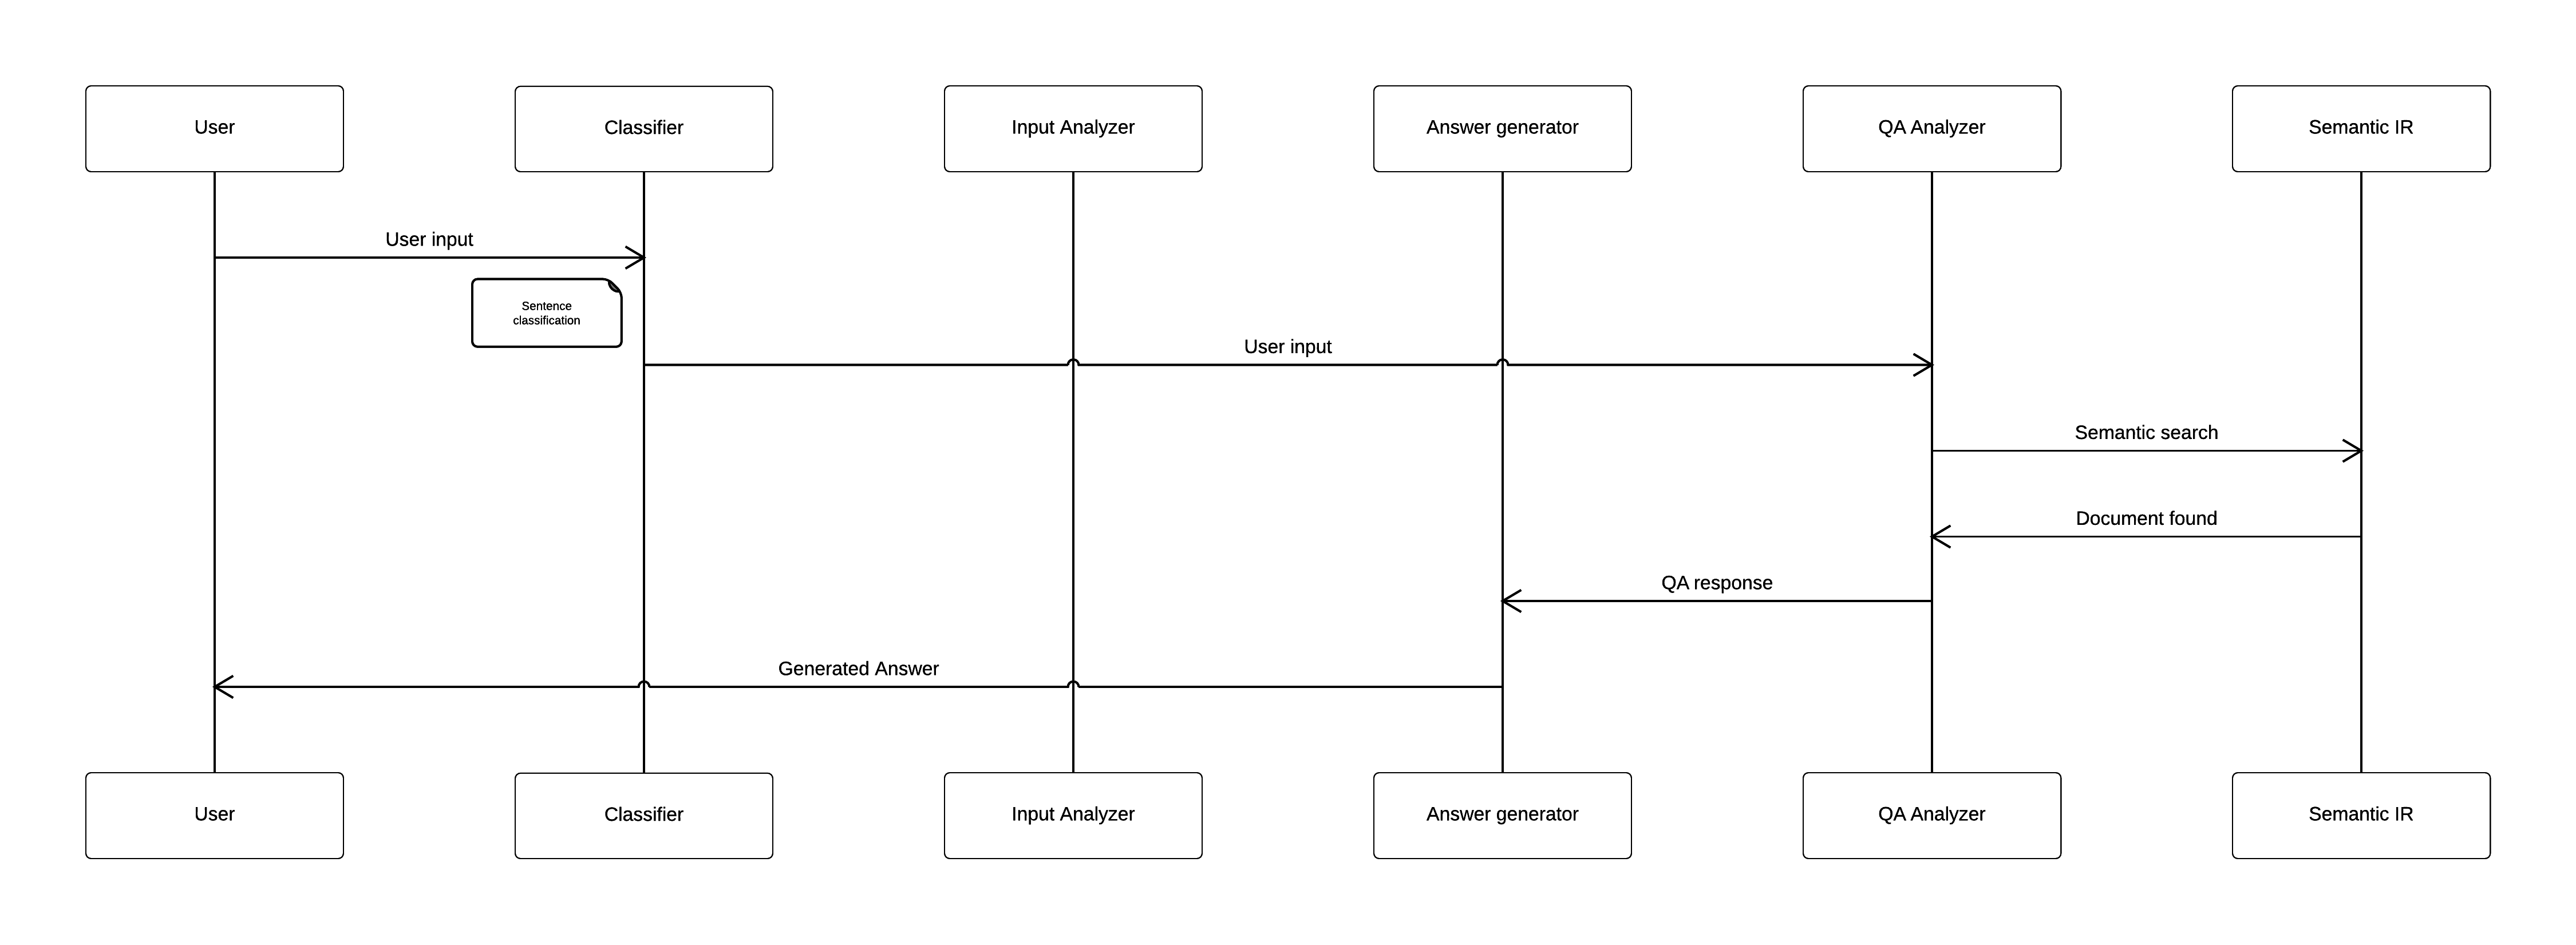
\includegraphics[width=\textwidth]{img/arch/FullQuestion.png}
    \caption{Question with \ac{KB} lookup process}
    \label{fig:arch3}
\end{figure}

% 
% Several things should go here:
%  * A description of how the system will behave when a question is received
%  * An UML (or several) describing that behaviour
%  * Something about PoS ?